\documentclass[aspectratio=169]{beamer}

\mode<presentation>
{
  \usetheme{default}
  \usecolortheme{default}
  \usefonttheme{default}
  \setbeamertemplate{navigation symbols}{}
  \setbeamertemplate{caption}[numbered]
  \setbeamertemplate{footline}[frame number]  % or "page number"
  \setbeamercolor{frametitle}{fg=white}
  \setbeamercolor{footline}{fg=black}
} 

\usepackage[english]{babel}
\usepackage[utf8x]{inputenc}
\usepackage{tikz}
\usepackage{courier}
\usepackage{array}
\usepackage{bold-extra}
\usepackage{minted}
\usepackage[thicklines]{cancel}
\usepackage{fancyvrb}

\xdefinecolor{dianablue}{rgb}{0.18,0.24,0.31}
\xdefinecolor{darkblue}{rgb}{0.1,0.1,0.7}
\xdefinecolor{darkgreen}{rgb}{0,0.5,0}
\xdefinecolor{darkgrey}{rgb}{0.35,0.35,0.35}
\xdefinecolor{darkorange}{rgb}{0.8,0.5,0}
\xdefinecolor{darkred}{rgb}{0.7,0,0}
\definecolor{darkgreen}{rgb}{0,0.6,0}
\definecolor{mauve}{rgb}{0.58,0,0.82}

\title[2018-07-25-codas-hep-ecosystem]{The Scientific Python Ecosystem}
\author{Jim Pivarski}
\institute{Princeton University -- DIANA-HEP}
\date{July 25, 2018}

\begin{document}

\logo{\pgfputat{\pgfxy(0.11, 7.4)}{\pgfbox[right,base]{\tikz{\filldraw[fill=dianablue, draw=none] (0 cm, 0 cm) rectangle (50 cm, 1 cm);}\mbox{\hspace{-8 cm}
\includegraphics[height=1 cm]{princeton-logo-long.png}
\includegraphics[height=1 cm]{diana-hep-logo-long.png}}}}}

\begin{frame}
  \titlepage
\end{frame}

\logo{\pgfputat{\pgfxy(0.11, 7.4)}{\pgfbox[right,base]{\tikz{\filldraw[fill=dianablue, draw=none] (0 cm, 0 cm) rectangle (50 cm, 1 cm);}\mbox{\hspace{-8 cm}
\includegraphics[height=1 cm]{princeton-logo.png}
\includegraphics[height=1 cm]{diana-hep-logo.png}}}}}

% Uncomment these lines for an automatically generated outline.
%\begin{frame}{Outline}
%  \tableofcontents
%\end{frame}

% START START START START START START START START START START START START START

\begin{frame}{Why you can't ignore Python}
\vspace{0.25 cm}
\begin{center}
\only<1>{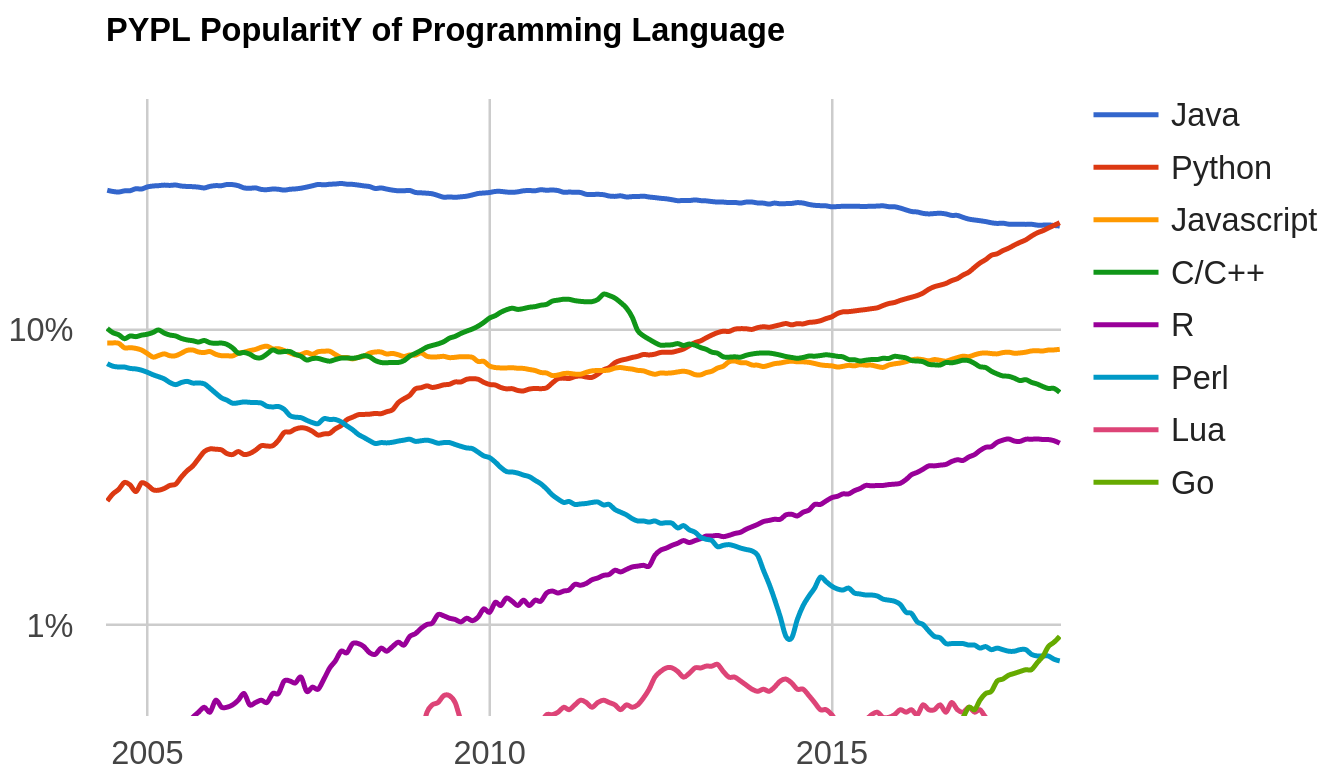
\includegraphics[width=0.8\linewidth]{pypl-popularity.png}}\only<2>{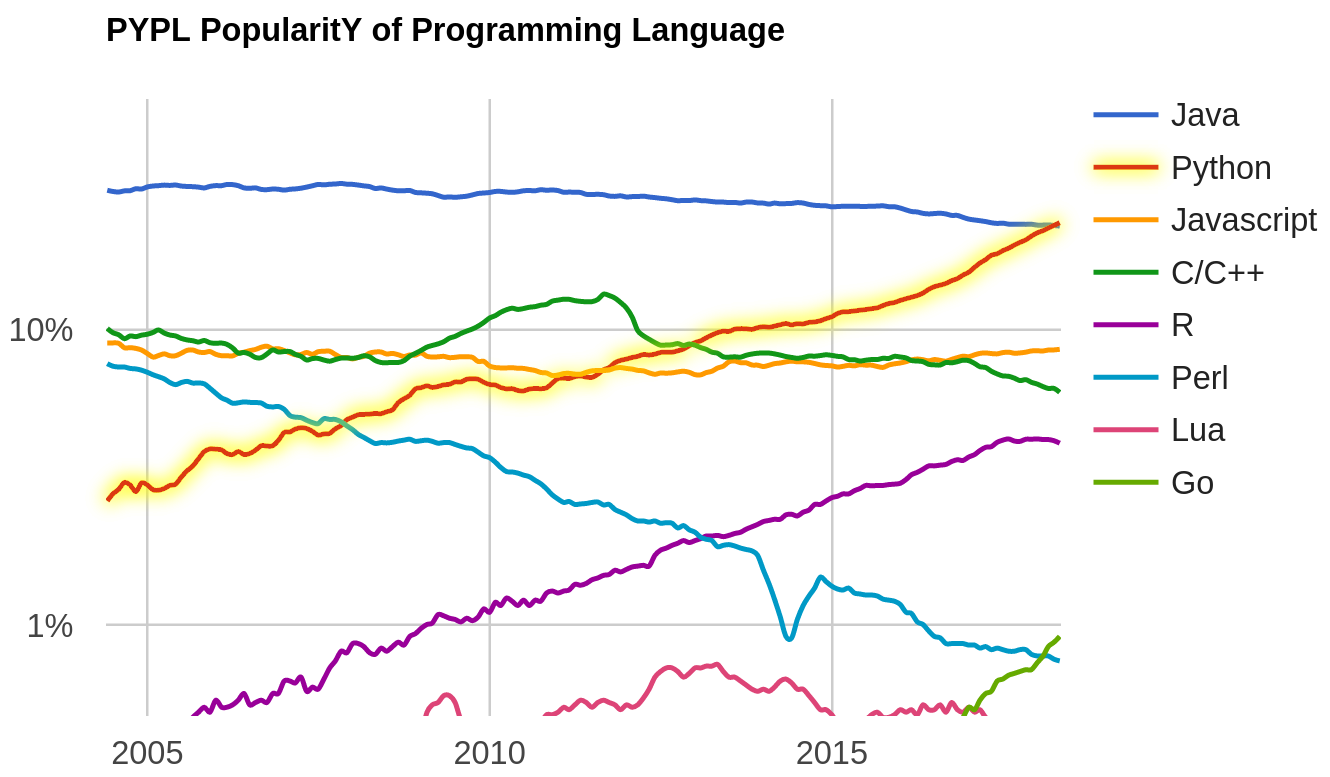
\includegraphics[width=0.8\linewidth]{pypl-popularity-2.png}}
\end{center}
\textcolor{blue}{\scriptsize\url{http://pypl.github.io/PYPL.html}}
\end{frame}

\begin{frame}{Why you can't ignore Python}
\vspace{0.5 cm}
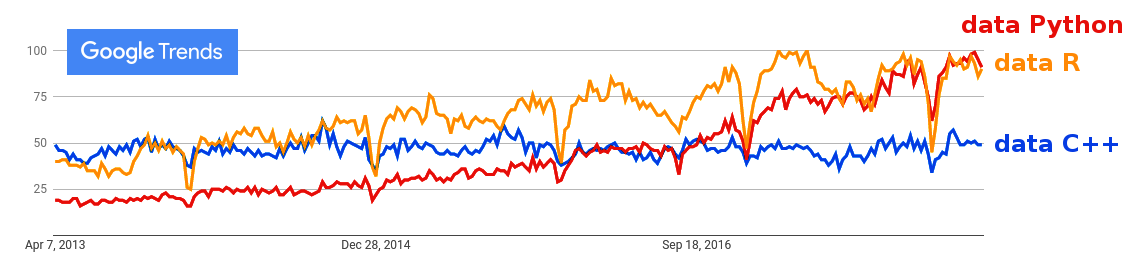
\includegraphics[width=\linewidth]{python-r-cpp-googletrends-data.png}

\vspace{1 cm}
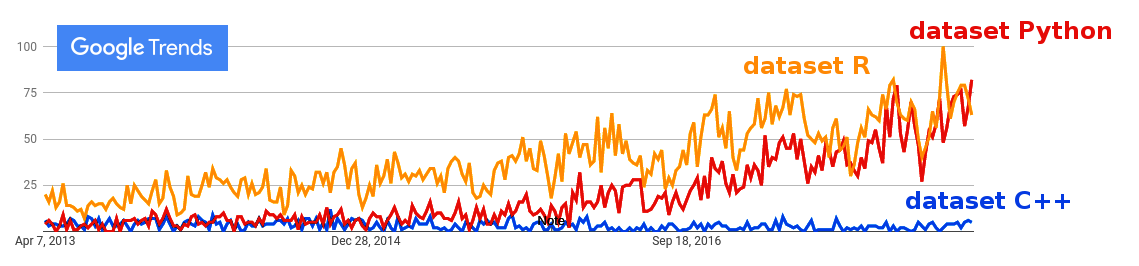
\includegraphics[width=\linewidth]{python-r-cpp-googletrends-dataset.png}
\end{frame}

\begin{frame}{Why you can't ignore Python}
\vspace{0.5 cm}
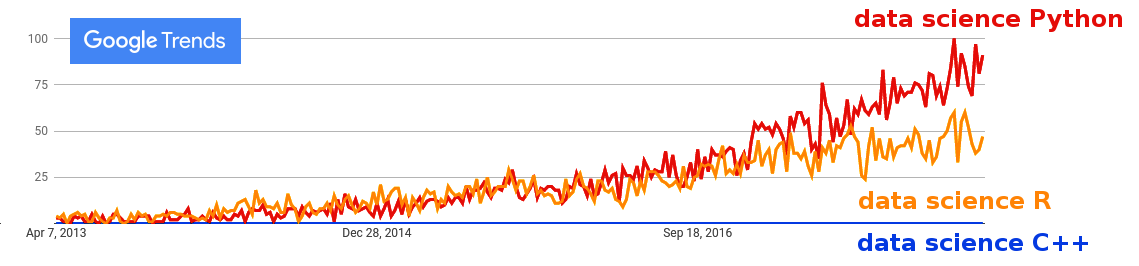
\includegraphics[width=\linewidth]{python-r-cpp-googletrends-datascience.png}

\vspace{1 cm}
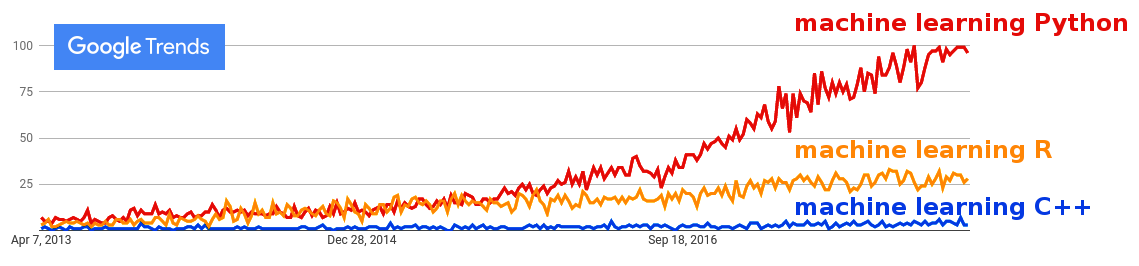
\includegraphics[width=\linewidth]{python-r-cpp-googletrends-machinelearning.png}
\end{frame}

\begin{frame}{Why you can't ignore Python}
\large
\vspace{0.4 cm}
All of the deep learning libraries I could find either have a Python interface or are primarily/exclusively Python.

\vspace{0.6 cm}
\mbox{ } 
\includegraphics[height=0.8 cm]{sklearn-logo.png}
\hfill 
\includegraphics[height=0.8 cm]{pytorch-logo.png}
\hfill 
\includegraphics[height=0.8 cm]{keras-logo.png}
\hfill 
\includegraphics[height=1 cm]{tensorflow-logo.png}
\hfill 
\includegraphics[height=0.8 cm]{caffe2-logo.png}
\hfill 
\includegraphics[height=0.8 cm]{gluon-logo.png} \mbox{ }

\vspace{0.45 cm}
\mbox{ } 
\includegraphics[height=0.8 cm]{chainer-logo.png}
\hfill 
\includegraphics[height=0.8 cm]{cntk-logo.png}
\hfill 
\includegraphics[height=0.8 cm]{lasagne-logo.png}
\hfill 
\includegraphics[height=0.8 cm]{onnx-logo.png}
\hfill 
\includegraphics[height=0.8 cm]{cesium-logo.png}
\hfill 
\includegraphics[height=0.8 cm]{xgboost-logo.png} \mbox{ }
\end{frame}

\begin{frame}{Why you can't ignore Python}
\vspace{0.25 cm}
\begin{center}
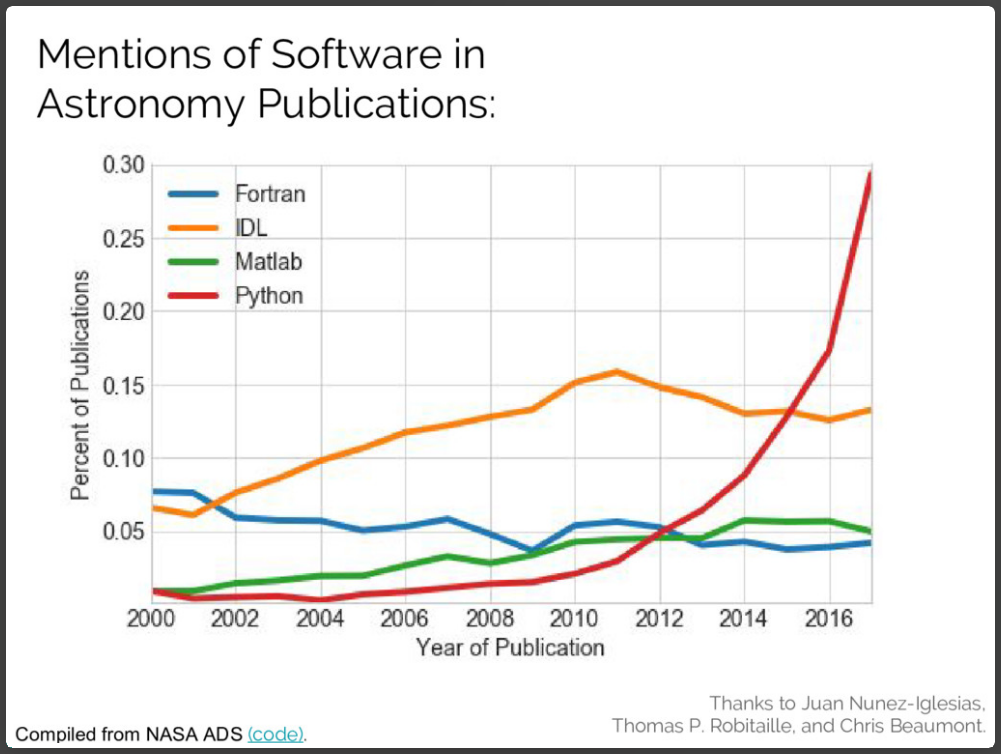
\includegraphics[width=0.7\linewidth]{mentions-of-programming-languages.png}
\end{center}
\end{frame}

\begin{frame}{More significant: what has grown around Python}
\vspace{0.25 cm}
\begin{columns}[b]
\column{0.75\linewidth}
\only<1>{
\includegraphics[height=7.8 cm]{shells-1.png}}
\only<2>{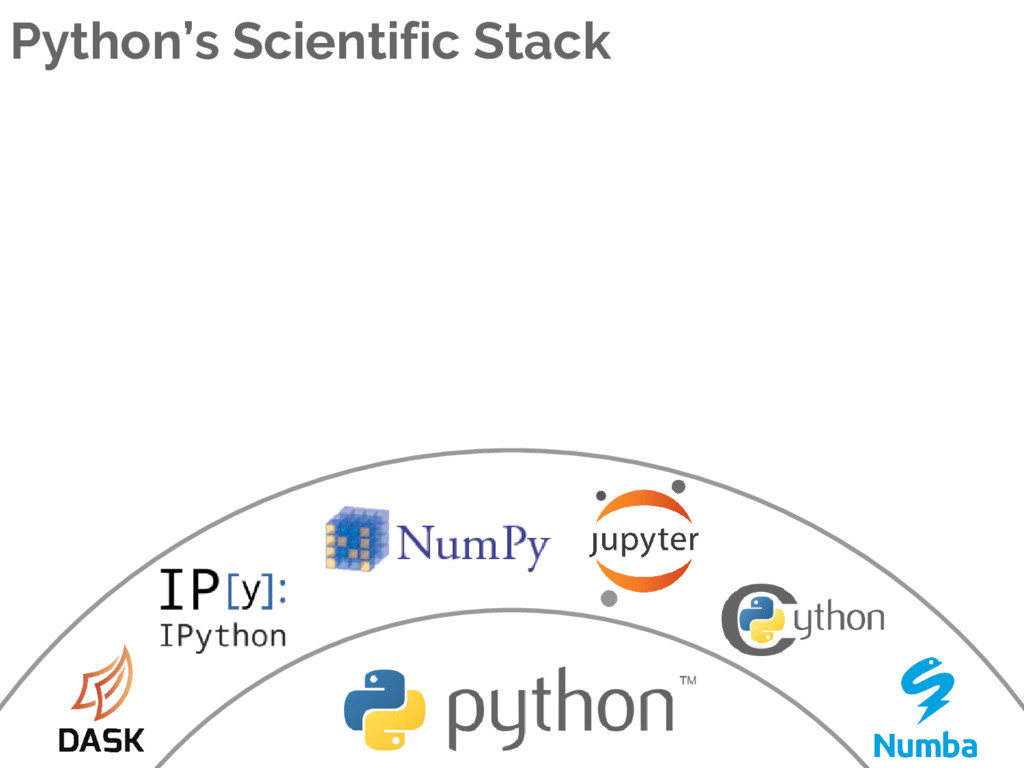
\includegraphics[height=7.8 cm]{shells-2.png}}
\only<3>{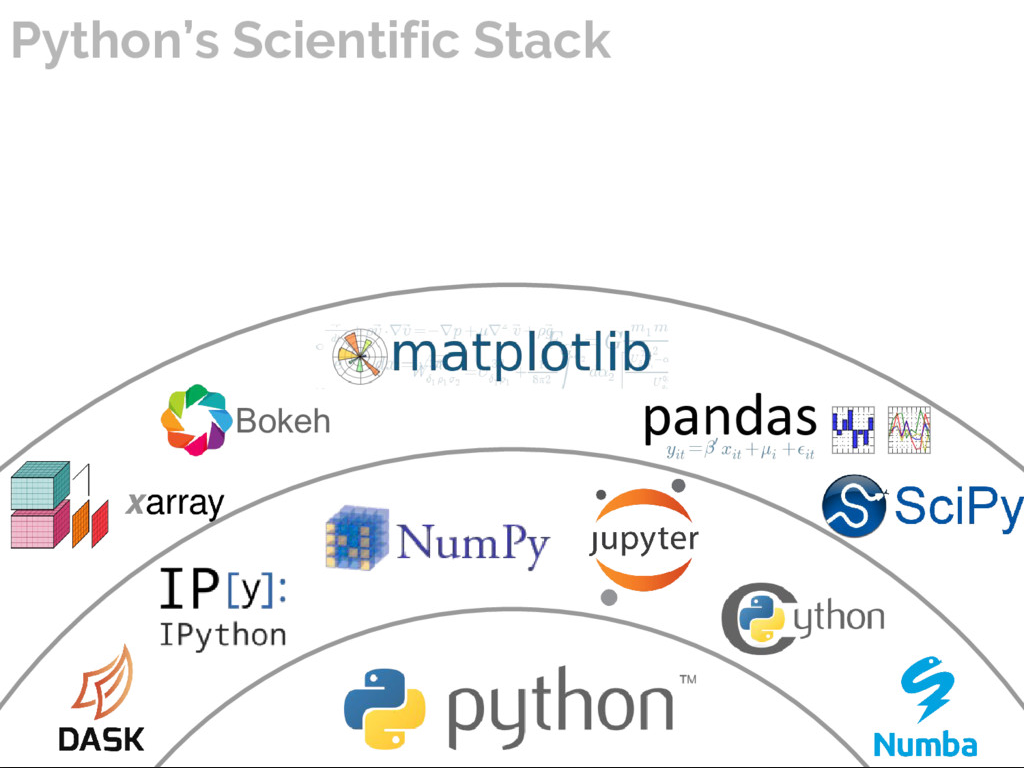
\includegraphics[height=7.8 cm]{shells-3.png}}
\only<4>{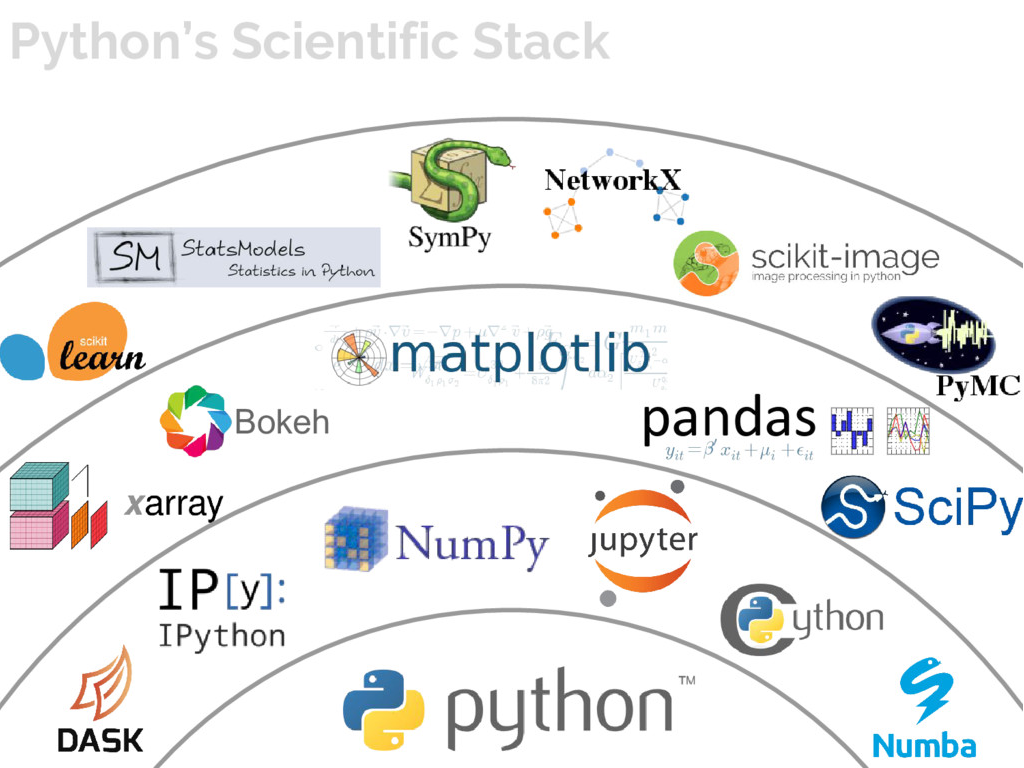
\includegraphics[height=7.8 cm]{shells-4.png}}
\only<5>{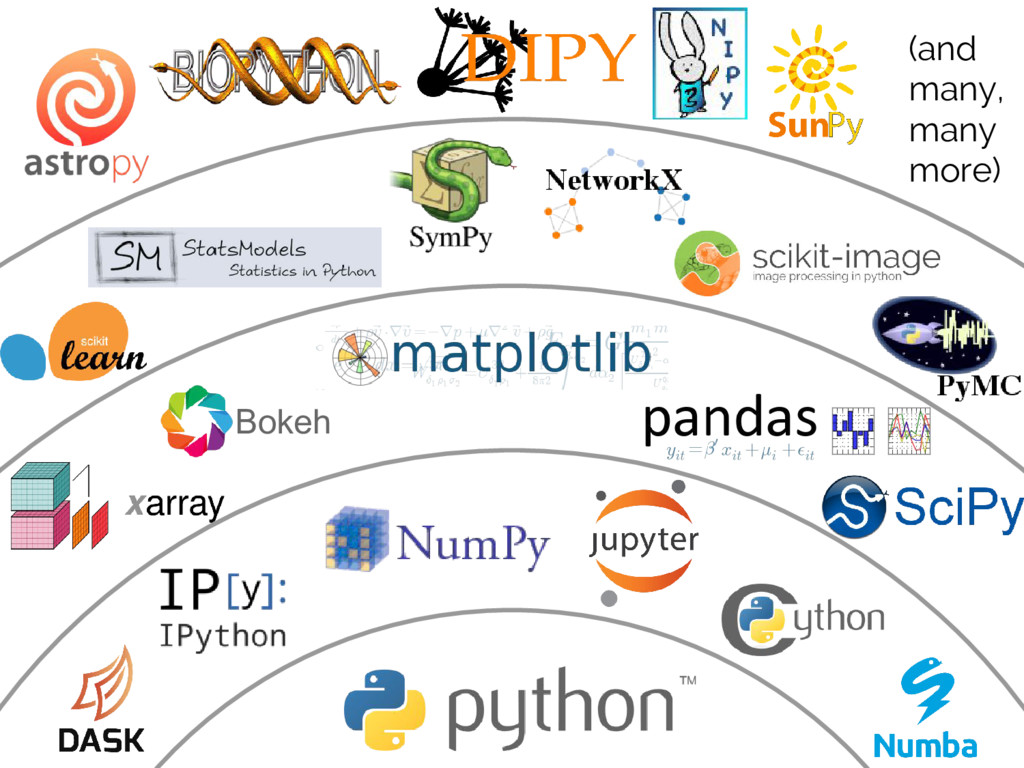
\includegraphics[height=7.8 cm]{shells-5.png}}

\column{0.25\linewidth}

\includegraphics[width=\linewidth]{unreasonable-effectiveness.png}
\vspace{5.3 cm}
\end{columns}
\end{frame}

\begin{frame}{Also stolen from that talk\ldots}
\vspace{0.1 cm}
\begin{columns}[b]
\column{0.75\linewidth}
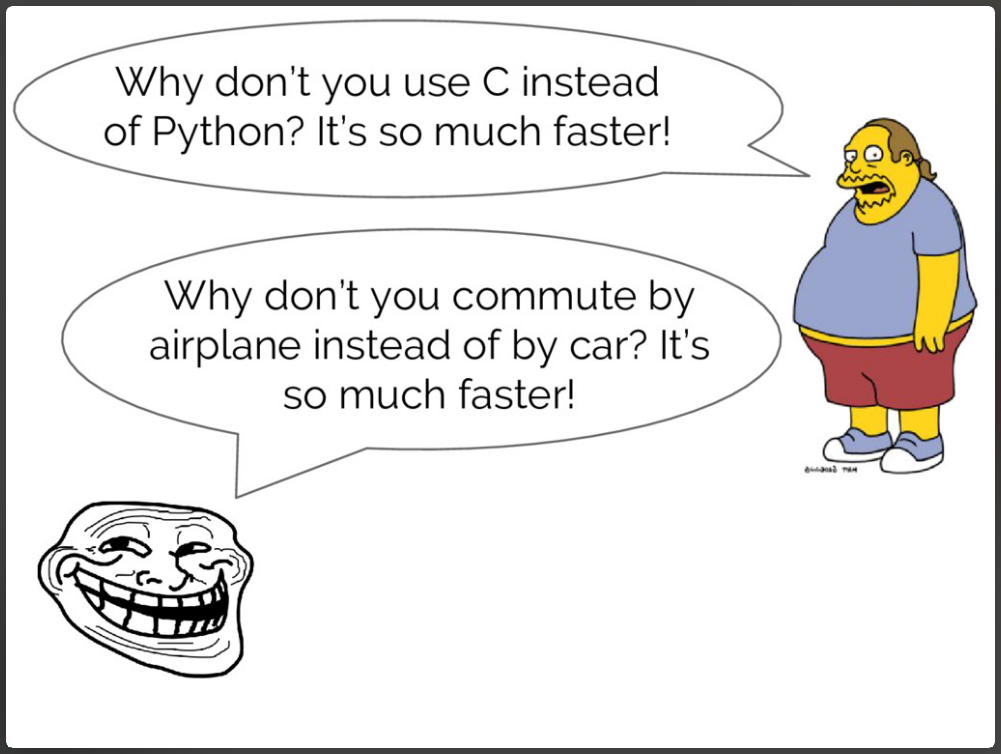
\includegraphics[height=7.8 cm]{commute-by-plane.png}
\column{0.25\linewidth}
\vspace{0.15 cm}

\includegraphics[width=\linewidth]{unreasonable-effectiveness.png}
\vspace{5.15 cm}
\end{columns}
\end{frame}

\begin{frame}{``Python is a slow language''}
\vspace{0.2 cm}
\begin{block}{Quibble: \textcolor{black}{A \underline{\it language} is neither fast nor slow. (But CPython is pretty slow.)}}
\end{block}

\begin{uncoverenv}<2->
\vspace{-0.2 cm}
\begin{block}{Why Python is slow}
\begin{itemize}
\item<3-> Virtual machine between Python bytecode and the physical machine.
\item<4-> Type-checking during execution, \underline{\it every time} in a tight for loop.
\item<5-> Data are bloated and distributed in memory \mbox{(cache line efficiency, pointer chasing).\hspace{-0.5 cm}}
\item<6-> Global Interpreter Lock (GIL): parallel processing is not parallel.
\end{itemize}
\end{block}
\end{uncoverenv}

\begin{uncoverenv}<7->
\begin{block}{Why Python is nevertheless good for science}
\begin{itemize}
\item<8-> Python usually just \underline{\it drives} compiled code (good C, C++, Fortran bindings).
\item<9-> Many \underline{\it standard} precompiled libraries, which also release the GIL.
\item<10-> \textcolor{darkorange}{\bf You start thinking in terms of ``slow control'' and ``fast math.''}
\item<11-> \textcolor{red}{\bf Computational performance is not the same as user productivity!}
\end{itemize}
\end{block}
\end{uncoverenv}
\end{frame}

\begin{frame}{Numpy was key to Python developing a scientific ecosystem}
\large
\vspace{0.1 cm}

\renewcommand{\arraystretch}{1.15}
\mbox{\hspace{-0.5 cm}\begin{tabular}{c p{0.95\linewidth}}
1994 & \textcolor{darkorange}{\bf Python} 1.0 released. \\
1995 & First array package: \textcolor{darkorange}{\bf Numeric} \textcolor{gray}{(a.k.a.\ Numerical, Numerical Python, NumPy).} \\
2001 & Diverse scientific codebases merged into \textcolor{darkorange}{\bf SciPy}. \\
2003 & \textcolor{darkorange}{\bf Matplotlib} \\
2003 & Numeric was limited; \textcolor{darkorange}{\bf numarray} appeared as a competitor with more \mbox{features} \textcolor{gray}{(memory-mapped files, alignment, record arrays)}. \\
2005 & Two packages were incompatible; could not integrate numarray-based code into SciPy. Travis Oliphant merged the codebases as \textcolor{red}{\bf Numpy}. \\
2008 & \textcolor{darkorange}{\bf Pandas} \\
2010 & \textcolor{darkorange}{\bf Scikit-Learn} \\
2011 & \textcolor{darkorange}{\bf AstroPy} \\
2012 & \textcolor{darkorange}{\bf Anaconda} \\
2014 & \textcolor{darkorange}{\bf Jupyter} \\
2015 & \textcolor{darkorange}{\bf Keras} \\
\end{tabular}}

\begin{uncoverenv}<2->
\vspace{-3 cm}
\hfill \fbox{\begin{minipage}{7 cm}
\vspace{0.2 cm}
\begin{center}
\begin{minipage}{6.5 cm}
The scientific Python ecosystem could have failed before it started if the Numeric-numarray split hadn't been resolved!
\end{minipage}
\vspace{0.2 cm}
\end{center}
\end{minipage}}
\end{uncoverenv}
\end{frame}

\begin{frame}[fragile]{The Numpythonic mindset}
\large
\vspace{0.5 cm}
Although you can write Python {\tt\normalsize for} loops over Numpy arrays, you don't reap the benefit unless you express your calculation in Numpy ufuncs (universal functions).

\vspace{\baselineskip}
\begin{columns}[t]
\column{0.45\linewidth}
\vspace{-\baselineskip}
\scriptsize
\begin{minted}{python}
pz = numpy.empty(len(pt))
for i in range(len(pt)):
    pz[i] = pt[i]*numpy.sinh(eta[i])
\end{minted}

\vspace{0.5 cm}
$\mathcal{O}(N)$ Python bytecode instructions, type-checks, interpreter locks.

\column{0.45\linewidth}
\mbox{\hspace{-0.85 cm}\textcolor{darkblue}{vs}}
\vspace{-\baselineskip}
\scriptsize
\begin{minted}{python}
pz = pt * numpy.sinh(eta)
\end{minted}
\vspace{2\baselineskip}

\vspace{0.5 cm}
$\mathcal{O}(1)$ Python bytecode instructions, type-checks, interpreter locks.

\vspace{0.1 cm}
$\mathcal{O}(N)$ statically typed, probably vectorized native bytecode operations on contiguous memory.
\end{columns}

\large
\vspace{0.75 cm}
\uncover<2->{\textcolor{darkorange}{\bf In other words, a \underline{S}ingle (Python) \underline{I}nstruction on \underline{M}ultiple \underline{D}ata.}}

\vspace{0.25 cm}
\uncover<3->{\textcolor{red}{\bf The same code reorganization that speeds up Python with Numpy would speed up C++ with CUDA or SIMD.}}
\end{frame}

\begin{frame}{The Numpythonic mindset: Numpy API in CUDA}
\vspace{0.35 cm}
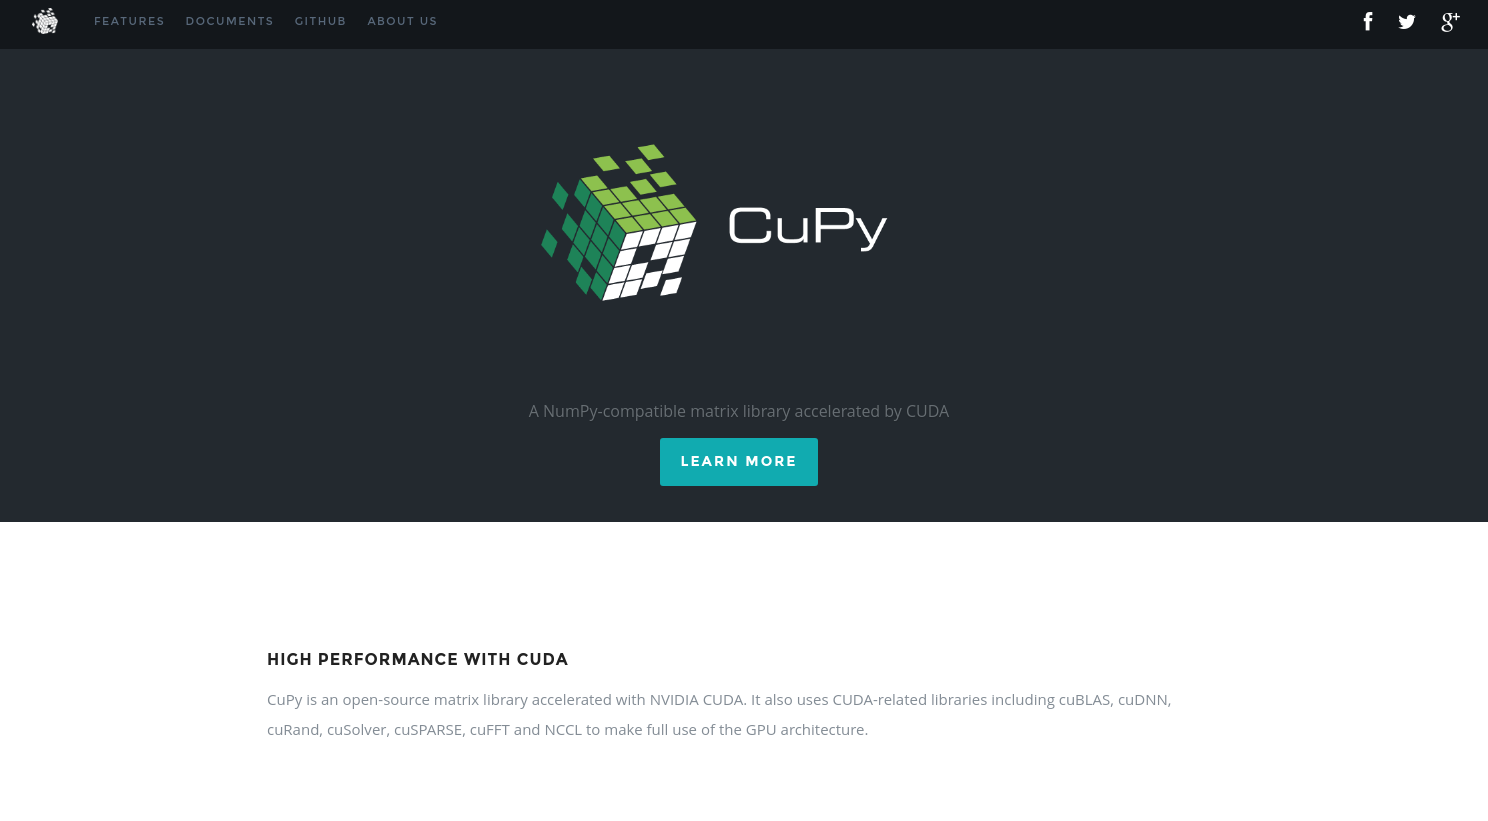
\includegraphics[width=\linewidth]{cupy.png}
\end{frame}

\begin{frame}{The Numpythonic mindset: Numpy API in C++}
\vspace{0.35 cm}
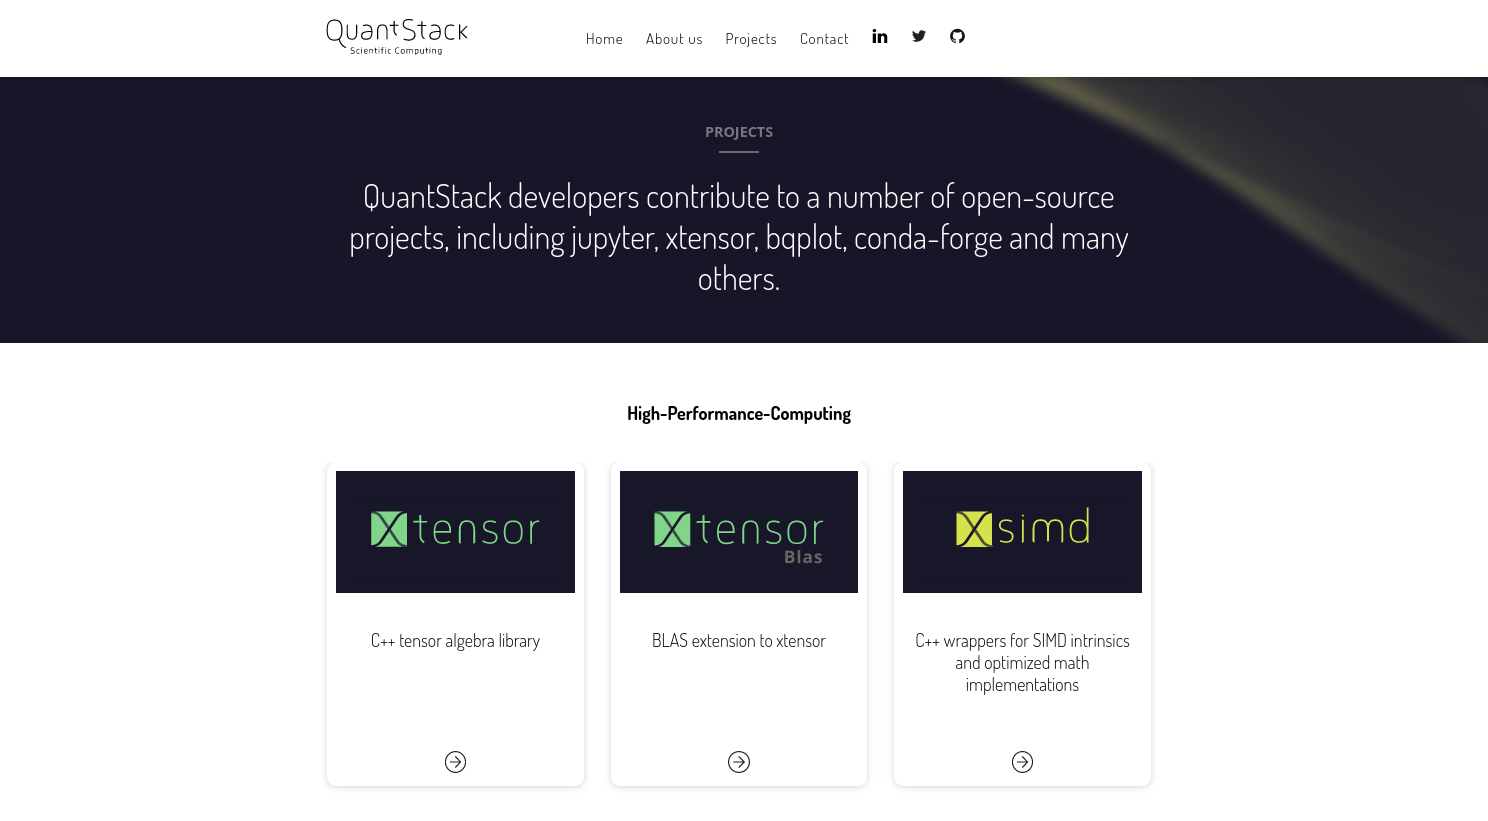
\includegraphics[width=\linewidth]{quantstack.png}
\end{frame}

\begin{frame}[fragile]{}
\huge
\vspace{0.5 cm}
\begin{center}
Switch to the notebooks now or install packages.

\large
\vspace{1 cm}
\begin{minipage}{0.35\linewidth}
\begin{minted}{bash}
# install Miniconda...
conda install pip
conda install numpy
pip install uproot
\end{minted}
\end{minipage}
\end{center}
\end{frame}


\end{document}

%% https://speakerdeck.com/jakevdp/the-unexpected-effectiveness-of-python-in-science
